%%%%%%%%%%%%%%%%%%%%%%%%%%%%%%%%%%%%%%%%%%%%%%%%%%%%%%%%%%%%%%%%%%%%%%%%%%%%%%%%
% test.tex
%%%%%%%%%%%%%%%%%%%%%%%%%%%%%%%%%%%%%%%%%%%%%%%%%%%%%%%%%%%%%%%%%%%%%%%%%%%%%%%%
%
% Authors:
% - Francois "fsechet" Sechet
%
%
%%%%%%%%%%%%%%%%%%%%%%%%%%%%%%%%%%%%%%%%%%%%%%%%%%%%%%%%%%%%%%%%%%%%%%%%%%%%%%%%

\documentclass{42}
\usepackage[T1]{fontenc}
\usepackage[utf8]{inputenc}
\usepackage{url}



%%%%%%%%%%%%%%%%%%%%%%%%%%%%%%%%%%%%%%%%%%%%%%%%%%%%%%%%%%%%%%%%%%%%%%%%%%%%%%%%
% Prologue
%%%%%%%%%%%%%%%%%%%%%%%%%%%%%%%%%%%%%%%%%%%%%%%%%%%%%%%%%%%%%%%%%%%%%%%%%%%%%%%%

\begin{document}

%Table des matieres
\title{Rubik}
\subtitle{Qu'est-ce que vous faites mercredi prochain ?}

\member {Fran\c{c}ois Sechet}{fsechet@student.42.fr}
\member {42 staff}{pedago@staff.42.fr}

\summary
{
	Ce projet va vous faire ecrire un programme qui resout des Rubik's Cubes en un minimum de mouvements.

}

\maketitle

\tableofcontents

% Valeurs utilisees pour la generation de headers d'exercices
\turnindir{svn+ssh://rendus@rendus.42.fr/sujetdetest-2142-login\_x}

\newpage
%%%%%%%%%%%%%%%%%%%%%%%%%%%%%%%%%%%%%%%%%%%%%%%%%%%%%%%%%%%%%%%%%%%%%%%%%%%%%%%%
% Start document
%%%%%%%%%%%%%%%%%%%%%%%%%%%%%%%%%%%%%%%%%%%%%%%%%%%%%%%%%%%%%%%%%%%%%%%%%%%%%%%%
\chapter{Pr\'eambule}

En soutenance, vous allez devoir faire mieux que \c{c}a :

\url{https://www.youtube.com/watch?v=eQH7MU0gUCQ}

\

A d\'efaut, ceci reste une performance acceptable :

\url{https://www.youtube.com/watch?v=_v85dcvw2vQ}

\

Par contre, \c{c}a, c'est trop facile :

\url{https://www.youtube.com/watch?v=X0pFZG7j5cE}

\newpage

%%%%%%%%%%%%%%%%%%%%%%%%%%%%%%%%%%%%%%%%%
%
% Introduction
%
%%%%%%%%%%%%%%%%%%%%%%%%%%%%%%%%%%%%%%%%%

\chapter{Introduction}

Tout le monde conna\^it le Rubik's Cube, et il y a de fortes chances pour que vous vous soyez d\'ej\`a un peu esquint\'e ce qui vous sert de cerveau dessus \`a un moment dans votre vie.

\

Que vous ayez ou non d\'ej\'a r\'eussi \`a le r\'esoudre, ce projet est \`a votre port\'ee de jeune programmeur enthousiaste. Il s'agit en effet d'un simple projet d'algorithmie, faisant un peu appel \`a de la repr\'esentation dans l'espace, \`a quelques vagues notions de th\'eorie des groupes, un peu aussi \`a votre cerveau, bref, des bricoles.

\

Dans ce projet, on vous demandera de r\'esoudre des Rubik's Cubes, selon les crit\`eres des comp\'etitions officielles de Rubik's Cube et en particulier celles du Fewest Moves Challenge (FMC), la limite de temps habituelle d'une heure en moins (votre limite de temps se comptera en secondes).

\

Lors d'une \'epreuve de FMC, tous les comp\'etiteurs sont enferm\'es dans une salle avec un papier, un stylo, un cube et c'est tout. Pendant soixante minutes, ils vont individuellement chercher la solution la plus courte au m\'elange donn\'e, et la rendre sur papier. Les solutions seront ensuite individuellement v\'erifi\'ees, et sera proclam\'e vainqueur celui avec le score le plus bas.

\

Bon courage !

\

\info
{
Le record du monde actuel de FMC est de 20 mouvements, par Tomoaki Okayama. Plus de 200 personnes ont d\'ej\'a trouv\'e des solutions en-dessous des 30 mouvements en comp\'etition.

D'autre part, il est prouv\'e que dans le pire des cas, pour chaque cube, il existe au moins une solution en au plus 20 mouvements. Plus d'informations: \url{http://www.cube20.org/}
}
\

\hint
{
Il est vivement encourag\'e d'apprendre \`a r\'esoudre le Rubik's Cube IRL pour ce projet.
}


%%%%%%%%%%%%%%%%%%%%%%%%%%%%%%%%%%%%%%%%%
%
% Definitions et syntaxe
%
%%%%%%%%%%%%%%%%%%%%%%%%%%%%%%%%%%%%%%%%%

\chapter{D\'efinitions et syntaxe}

Votre programme doit accepter en param\`etre le chemin vers un fichier contenant un ou plusieurs m\'elanges s\'epar\'es par un saut de ligne.

\

Un m\'elange est une s\'equence de mouvements s\'epar\'es par un ou plusieurs espaces \`a appliquer sur un cube de mani\`ere \`a le m\'elanger non pas al\'eatoirement mais selon un pattern pr\'ed\'efini.

\

La notation utilis\'ee est la notation internationale (F R U B L D pour Front / Right / Up / Back / Left / Down). Pour comprendre cette notation, je vous redirige vers \url{http://www.francocube.com/notation.php} qui me semble \^etre un bon point de d\'epart, le reste du site \'etant \'egalement tr\`es riche d'enseignements pour ce projet. Je vous invite \'egalement \`a bien regarder la vid\'eo de ce projet.

\
\hint
{
Une notation alternative existe, d'origine belge. Son utilisation est source de beaucoup de confusion, ce qui explique son manque de succ\`es au niveau international. Vous ne devez pas l'utiliser pour ce projet. La voici :
D D D D D D pour Dessus / Dessous / Devant / Derri\`ere / Droite / De l'autre c\^ot\'e.
}

\
F R U B L D repr\'esente \`a la fois une face et un mouvement appliqu\'e \`a cette face, mais la nuance est g\'en\'eralement assez explicite. Vos programmes doivent accepter les modificateurs de mouvements ' et 2 et renvoyer une solution utilisant cette m\^eme notation.

\

Voici un exemple de s\'equence valide :
R2 D' B' D F2 R F2 R2 U L' F2 U' B' L2 R D B' R' B2 L2 F2 L2 R2 U2 D2

\
\warn
{
Les mouvements de tranches M, E et S ainsi que les rotations x, y et z ne sont pas accept\'es.
}

\newpage
%%%%%%%%%%%%%%%%%%%%%%%%%%%%%%%%%%%%%%%%%
%
% Sujet - Partie obligatoire
%
%%%%%%%%%%%%%%%%%%%%%%%%%%%%%%%%%%%%%%%%%

\chapter{Sujet - Partie obligatoire}

Votre programme doit retourner sur la sortie standard les s\'equences de mouvements \`e appliquer sur un cube de type 3x3x3 pr\'ealablement m\'elang\'e avec la(les) s\'equence(s) donn\'ee(s) contenue(s) dans un fichier texte. Si le fichier contient plusieurs m\'elanges, votre programme les retournera l'un apr\`es l'autre, dans l'ordre, chacun suivi d'un '\textbackslash n'.

\

Par exemple:
\begin{42console}
$>./rubik fmc.txt | cat -e
$>B2 R' U B' U2 F B L U R D F D F' U' F2 U2 L' R D' R U' D2 B2 R' D2 B' U2 L B D R2 U F2 U D B L F' L$
L R' U' R' B' R L' F2 L U' L F' B' L2 R' D R2 B2 D2 F' B D2 B' F2 U R' D R2 D U' B L2 U F U2 L' D' U' R D B' R$
U' F2 D' R2 U' D2 R B2 F2 U' L' B' R2 B' D' R' D' U F' R2 D2 F R' B' F2 L R D' B F2 R2 F2 B R2 U' L R'$
\end{42console}

\

Retourner l'inverse du m\'elange (ou variante directe avec insertion de s\'equences sans effet pour en modifier la longueur) s'apparente grandement \`a un cas de triche...

\

Vous devrez comme toujours g\'erer les erreurs de mani\`ere sensible.

\

La m\'etrique utilis\'ee pour compter les mouvements est une m\'etrique par demi-tour (HTM), \`a savoir qu'un quart de tour ou demi-tour sur une m\^eme face comptent pour un seul mouvement, mais les mouvements de tranches comptent pour deux mouvements. Bref, votre score sera le r\'esultat d'un wc -w sur votre solution.

\

\begin{42console}
$> ./rubik fmc.txt | wc -w
      42
\end{42console}

\newpage


%%%%%%%%%%%%%%%%%%%%%%%%%%%%%%%%%%%%%%%%%
%
% Sujet - Partie obligatoire
%
%%%%%%%%%%%%%%%%%%%%%%%%%%%%%%%%%%%%%%%%%


\chapter{Sujet - Partie bonus}

Tant que les contraintes de la partie obligatoire et des consignes sont respect\'ees, vous pouvez ajouter tous les bonus que vous souhaitez, qui seront jug\'es \`a la discr\'etion de vos correcteurs.

\

Par exemple :

\
\begin{itemize}
	\item Une vraie repr\'esentation graphique de l'\'etat du cube \`a intervalles r\'eguliers (ncurses, minilibx, openGL? ce que vous voulez - une simple s\'erie de chiffres ou de lettres est consid\'er\'e comme du debug, pas vraiment comme un r\'eel bonus...), voire une repr\'esentation visuelle des faces qui tournent en temps r\'eel (\c{c}a c'est vraiment classe !)
	\item Un algorithme qui descend aux fronti\`eres des solutions les plus optimales dans un d\'elai qui reste raisonnable (au-del\`a de quelques secondes, ce n'est plus raisonnable)
	\item Un choix entre plusieurs algorithmes, voire une s\'election de la meilleure solution entre plusieurs algorithmes
	\item Un g\'en\'erateur de m\'elanges int\'egr\'e dont on peut sp\'ecifier la longueur et/ou le nombre
	\item Une subdivision de votre solution en sous-\'etapes "humainement compr\'ehensibles"
	\item Un fonctionnement avec d'autres puzzles (4x4x4, 2x2x2, Megaminx, Square-1?)
	\item De r\'eelles performances du corrig\'e \`a la r\'esolution d'un rubik's cube en soutenance
	\item ...
\end{itemize}
\
\\
Les bonus ne seront comptabilis\'es que si la partie obligatoire est parfaitement r\'eussie.

\

Ces bonus ne doivent pas outrepasser le fonctionnement normal du programme (i.e. l'input des m\'elanges doit toujours \^etre un fichier quelconque dont on sp\'ecifie le chemin en premier param\`etre de votre ex\'ecutable), d'\'eventuelles options pr\'ealables peuvent \^etre indiqu\'ees pr\'ec\'ed\'ees d'un '-'.


%%%%%%%%%%%%%%%%%%%%%%%%%%%%%%%%%%%%%%%%%
%
% Sujet - Partie obligatoire
%
%%%%%%%%%%%%%%%%%%%%%%%%%%%%%%%%%%%%%%%%%

\chapter{Consignes}
Ce projet sera corrig\'e uniquement par des humains.

\

Vous \^etes libre d'utiliser le langage de votre choix (C, C++, Perl, Python, Java, Brainfuck si \c{c}a vous amuse?). Si une norme est impos\'ee pour le langage que vous choisissez, vous devrez la respecter scrupuleusement. Aucun segfault, fuite m\'emoire, double free, boucle infinie, interruption non g\'er\'ee avec discernement ne seront tol\'er\'es, \`a plus forte raison parce que ce n'est clairement pas le plus difficile dans ce projet.

\

Le cas \'ech\'eant, vous devrez fournir un Makefile avec les r\`egles habituelles pour compiler votre programme.

\

Vous avez le droit d'utiliser toute librairie que vous pouvez justifier en soutenance. Bien entendu, toute utilisation d'une librairie ou ressource externe faisant vraiment le boulot \`a votre place n'est pas autoris\'ee, vous devez justifier votre propre algorithme en correction.

\

Vous devez \^etre en mesure d'expliquer votre algorithme avec des mots et des concepts visuels simples. 

\

Les correcteurs seront particuli\`erement vigilants aux cas de triche qui entra\^inent syst\'ematiquement, dans les comp\'etitions officielles de Rubik's Cube, le bannissement de toute comp\'etition pendant plusieurs ann\'ees. A 42, nous nous contenterons de simples s\'eances d'humiliation publique et de la fourniture de sucreries pour tout le cluster.

\

Contrairement \`a vos coll\`egues en comp\'etition de FMC, vous avez le droit de vous aider de google, de vos voisins de gauche ET de droite ou du forum. Mais \`a l'instar de vos coll\`egues en comp\'etition de FMC, essayez de vous servir prioritairement de votre cerveau...


\chapter{Premier chapitre}

\section{Section premiere}

\subsection{Sous-section the first}

\begin{itemize}
	\item Liste
	\item de
	\item trucs
	\begin{itemize}
		\item nested
		\item trop bien
	\end{itemize}
	\item mais j'aime les poneys
\end{itemize}


\begin{figure}[ht!]
  \centering
  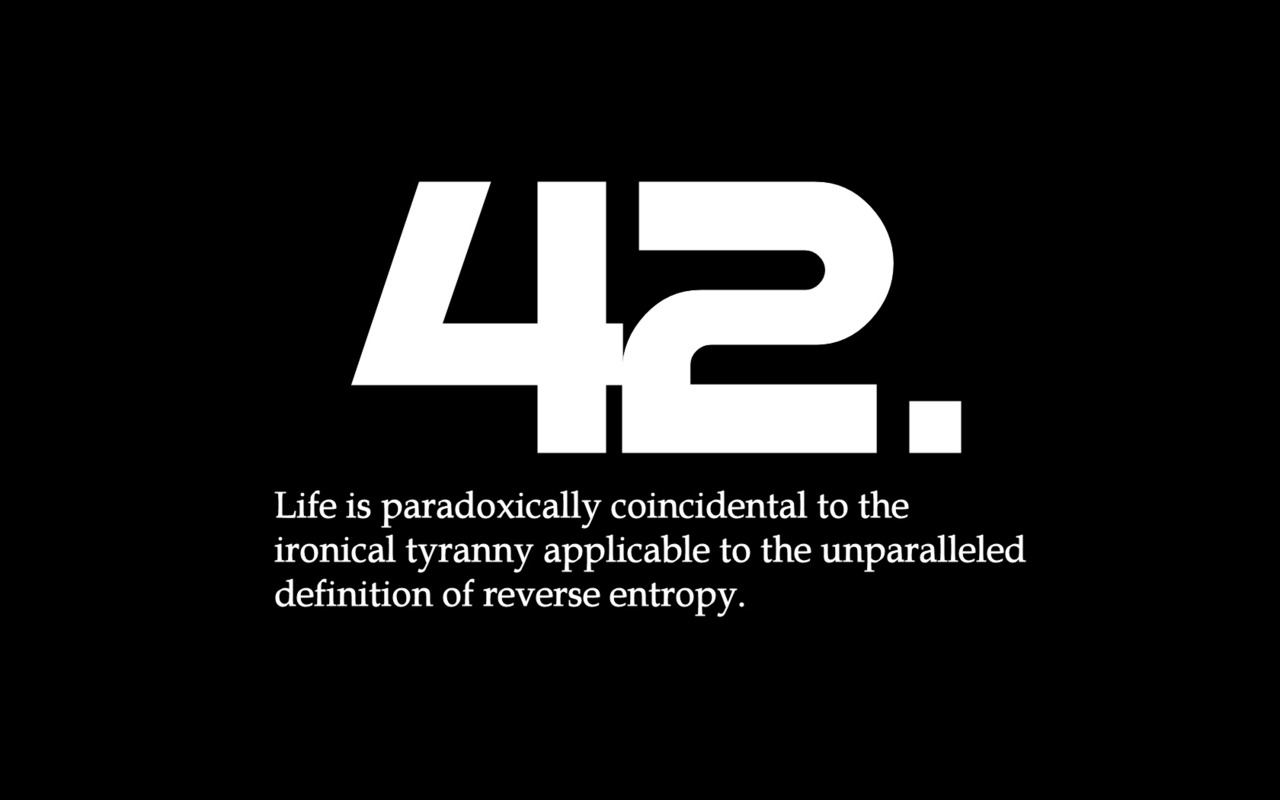
\includegraphics[width=90mm]{42.jpg}
\end{figure}


\newpage

\begin{42ccode}
/* Awesome code is awesome */
int		main(int ac, char** av)
{
	my_putstr("J'aime le 101010");
        return 0;
}
\end{42ccode}

\begin{42console}
$>ls
Makefile  test.aux  test.log  test.outtest.pdf  test.tex  test.toc
$>
\end{42console}


\hint
{
	Hint box
}

\warn
{
	Warn box
}

\info
{
	Info box
}

\chapter{Ceci est un exercice}

\extitle{Ceci est le titre de l'exercice}
\exnumber{00}
\exscore{42}
\exfiles{tamere.h,tamere.c}

\makeheaderbasic

Ceci est le sujet de l'exercice.

%%%%%%%%%%%%%%%%%%%%%%%%%%%%%%%%%%%%%%%%%%%%%%%%%%%%%%%%%%%%%%%%%%%%%%%%%%%%%%%%
% End document
%%%%%%%%%%%%%%%%%%%%%%%%%%%%%%%%%%%%%%%%%%%%%%%%%%%%%%%%%%%%%%%%%%%%%%%%%%%%%%%%
\end{document}
